\documentclass{article}

% 导入宏包
\usepackage{fancyhdr}
\usepackage{ctex}
\usepackage{listings}
\usepackage{graphicx}
\usepackage[a4paper, body={18cm,22cm}]{geometry}
\usepackage{amsmath,amssymb,amstext,wasysym,enumerate,graphicx}
\usepackage{float,abstract,booktabs,indentfirst,amsmath}
\usepackage{array}
\usepackage{multirow}
\usepackage{url}
\usepackage{diagbox}
\usepackage{enumitem}
\usepackage{xcolor}
\usepackage{makecell}
\usepackage{tikz}
\usetikzlibrary{positioning, arrows.meta}

% 设置段落
\renewcommand\arraystretch{1.4}
\setlength{\parindent}{2em}
\setCJKmonofont{黑体}

% 配置代码显示
\lstset{
	xleftmargin = 3em,
	xrightmargin = 3em,
	aboveskip = 1em,
	backgroundcolor = \color{white},
	basicstyle = \small\ttfamily,
	rulesepcolor = \color{gray},
	breaklines = true,
	numbers = left,
	numberstyle = \small,
	numbersep = -14pt,
	keywordstyle = \color{purple}\bfseries,
	commentstyle = \color{green!60!black}, % 修改注释颜色
	stringstyle = \color{red!60!green!90!blue!90},
	morekeywords = {ASSERT, int64_t, uint32_t},
	moreemph = {ASSERT, NULL},
	emphstyle = \color{red}\bfseries,
	moreemph = [2]{int64\_t, uint32\_t, tid\_t, uint8\_t, int16\_t, uint16\_t, int32\_t, size\_t, bool},
	emphstyle = [2]\color{purple}\bfseries,
	frame = shadowbox,
	showspaces = false,
	columns = fixed
	morecomment = [l][\color{green!60!black}]{+}, % 设置以+开头的代码行为绿色
}

%--------------------页眉--------------------%

\pagestyle{fancy}
\fancyhead[L]{}
\fancyhead[R]{}
\fancyhead[C]{华东师范大学软件工程学院实验报告}
\fancyfoot[C]{-\thepage-}
\renewcommand{\headrulewidth}{1.5pt}

%--------------------标题--------------------%

\begin{document}
	\begin{center}
		{\Large{\textbf{\heiti 华东师范大学软件工程学院实验报告}}}
		\begin{table}[htb]
			\flushleft
			\begin{tabular}{p{0.4\linewidth}p{0.27\linewidth}p{0.28\linewidth}}\\
				\textbf{实验课程}:计算机网络实践  & \textbf{年级}:2023级       & \textbf{实验成绩}:  \\
				\textbf{实验名称}:Protocol Layer & \textbf{姓名}:顾翌炜         &                 \\
				\textbf{实验编号}:Lab-1     & \textbf{学号}:10235101527 & \textbf{实验日期}:2024/11/15  \\
				\textbf{指导教师}:王廷     & \textbf{组号}:01            & \textbf{实验时间}:2024/11/15  \\ 
			\end{tabular}
		\end{table}
	\end{center}
	\rule{\textwidth}{2pt}
	
	%--------------------正文--------------------%
	\section{实验目的}
	
	\begin{enumerate}[noitemsep, label={{\arabic*})}]
		\item 学会通过Wireshark获取各协议层的数据包
		\item 掌握协议层数据包结构
		\item 分析协议开销
	\end{enumerate}
	
	\section{实验内容与实验步骤}
	
	\subsection{实验内容}
	
	\subsubsection{获取协议层的数据包}
	使用\texttt{wget}命令发起\texttt{HTTP}请求,然后使用\texttt{Wireshark}进行抓包。
	
	\subsubsection{绘制数据包结构}
	
	分析\texttt{HTTP} \texttt{GET}协议包的内容,并绘制协议包,分别标出\texttt{Ethernet},\texttt{IP}和\texttt{TCP}协议的头部的位置、大小以及其负载的范围。
	
	\subsubsection{分析协议开销}
	
	根据实验结构,分析\texttt{HTTP}应用协议额外开销。
	估计上面捕获的\texttt{HTTP}协议的额外开销。
	假设\texttt{HTTP}数据(头部和消息)是有用的,而\texttt{TCP},\texttt{IP}和\texttt{Ethernet}头部认为是开销。对于下载的主要部分中的每一个包,我们需要分析\texttt{Ethernet},\texttt{IP}和\texttt{TCP}的开销,和有用的\texttt{HTTP}数据的开销。根据以上的定义来估计下载协议的开销,来判定这种开销是否有必要。
	
	\subsubsection{分析解复用键}
	
	\textbf{解复用}指的是找到正确的上一层协议来处理到达的包。
	
	观察下载的以太网和\texttt{IP}包的头部信息,回答下面问题:
	
	\begin{enumerate}[noitemsep]
		\item Which Ethernet header field is the demultiplexing key that tells it the next higher layer is IP? What value is used in this field to indicate \textbf{“IP”}?
		\item Which IP header field is the demultiplexing key that tells it the next higher layer is TCP? What value is used in this field to indicate \textbf{“TCP”}?
	\end{enumerate}
	
	\subsubsection{问题讨论}
	
	\textbf{Explore on your own:}
	
	\begin{enumerate}[noitemsep]
		\item Look at a short TCP packet that carries no higher-layer data. To what entity is this packet destined? After all, if it carries no higher-layer data then it does not seem very useful to a higher layer protocol such as HTTP!
		\item In a classic layered model, one message from a higher layer has a header appended by the lower layer and becomes one new message. But this is not always the case. Above, we saw a trace in which the web response (one HTTP message comprised of an HTTP header and an HTTP payload) was converted into multiple lower layer messages (being multiple TCP packets).  Imagine that you have drawn the packet structure (as in step 2) for the first and last TCP packet carrying the web response.  How will the drawings differ?
		\item In the classic layered model described above, lower layers append headers to the messages passed down from higher layers. How will this model change if a lower layer adds encryption?
		\item In the classic layered model described above, lower layers append headers to the messages passed down from higher layers. How will this model change if a lower layer adds compression?
	\end{enumerate}
	
	
	\subsection{实验步骤}
	
	\begin{enumerate}[noitemsep, label={{\arabic*})}]
		\item 安装实验所需软件(为方便安装,我们使用\texttt{Windows}下的包管理器\texttt{winget})
		
		\begin{lstlisting}[language=bash]
        C:\User\GHOST> winget install wget
		\end{lstlisting}
		
		\begin{figure}[H]
			\centering
			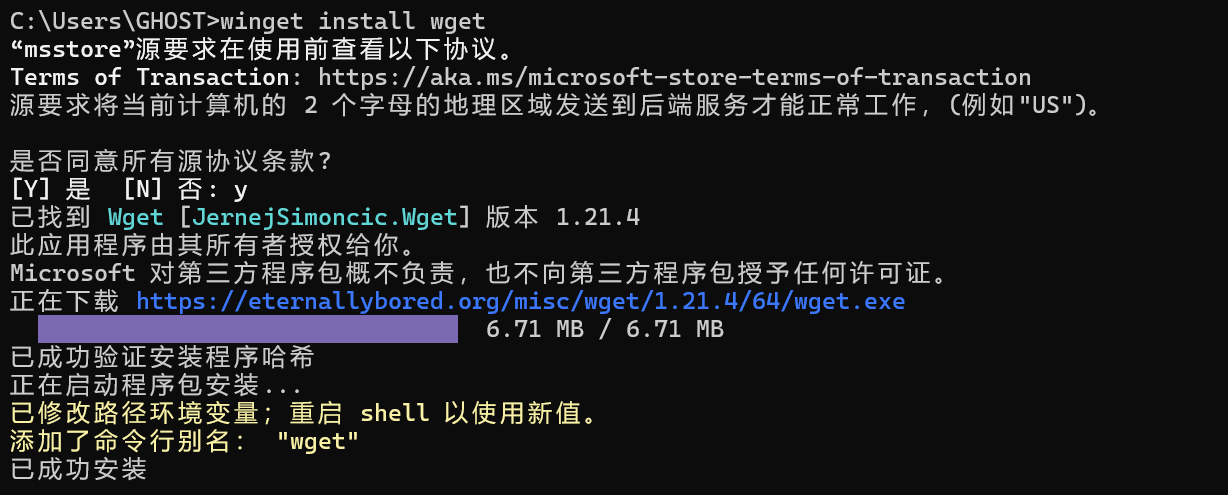
\includegraphics[width=12cm]{images/1.下载wget.png}
			\caption{下载wget}
		\end{figure}
		
		并从官网按照步骤下载wireshark软件
		
		\item 打开\texttt{Wireshark},在菜单栏的 \texttt{捕获 -> 选项} 中进行设置,选择已连接的网络,设置捕获过滤器为\texttt{tcp port 80},将混杂模式设为关闭,勾选 \texttt{enable network  name resolution},然后开始捕获。
		\item 使用 \texttt{wget} 命令发起 \texttt{HTTP} 请求
		\begin{lstlisting}[language=bash]
        C:\User\GHOST> wget http://www.baidu.com
		\end{lstlisting}
		\item 在 \texttt{Wireshark} 中停止捕获。
		\item 分析\texttt{HTTP} \texttt{GET}协议包的内容,并绘制协议包。
		\item 分析协议开销
		\item 分析解复用键
		\item 问题讨论
	\end{enumerate}
	
	\section{实验环境}
	
	\begin{itemize}[noitemsep]
		\item 操作系统:\texttt{Windows 11 家庭中文版 23H2 22631.4460}
		\item 网络适配器:\texttt{Killer(R)Wi-Fi 6E AX1675i 160MHz Wireless Network Adapter(211NGW)}
		\item \texttt{Wireshark}:\texttt{Version 4.4.1}
		\item \texttt{wget}:\texttt{GNU Wget 1.21.4 built on mingw32}
	\end{itemize}
	
	\section{实验过程与分析}
	
	\subsection{获取协议层的数据包}
	
	首先,我们打开\texttt{Wireshark},在菜单栏的 \texttt{捕获 -> 选项} 中进行设置,选择已连接的网络,设置捕获过滤器为\texttt{tcp port 80},将混杂模式设为关闭,勾选 \texttt{enable network  name resolution},然后开始捕获。
	
	\begin{figure}[H]
		\centering
		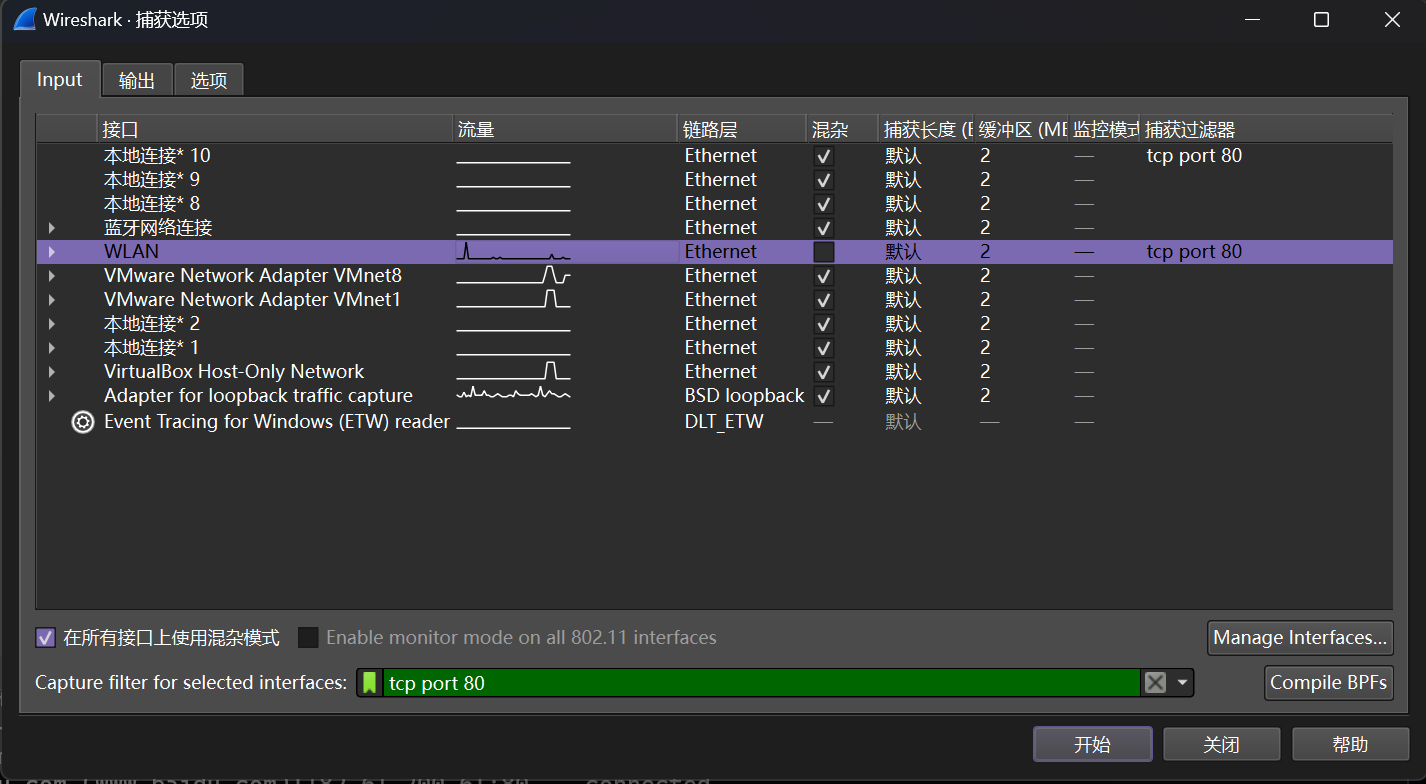
\includegraphics[width=11cm]{images/2.设置捕获.png}
		\caption{设置捕获}
	\end{figure}
	
	然后,我们使用 \texttt{wget} 命令对\texttt{http://www.baidu.com}发起 \texttt{HTTP} 请求
	
	\begin{figure}[H]
		\centering
		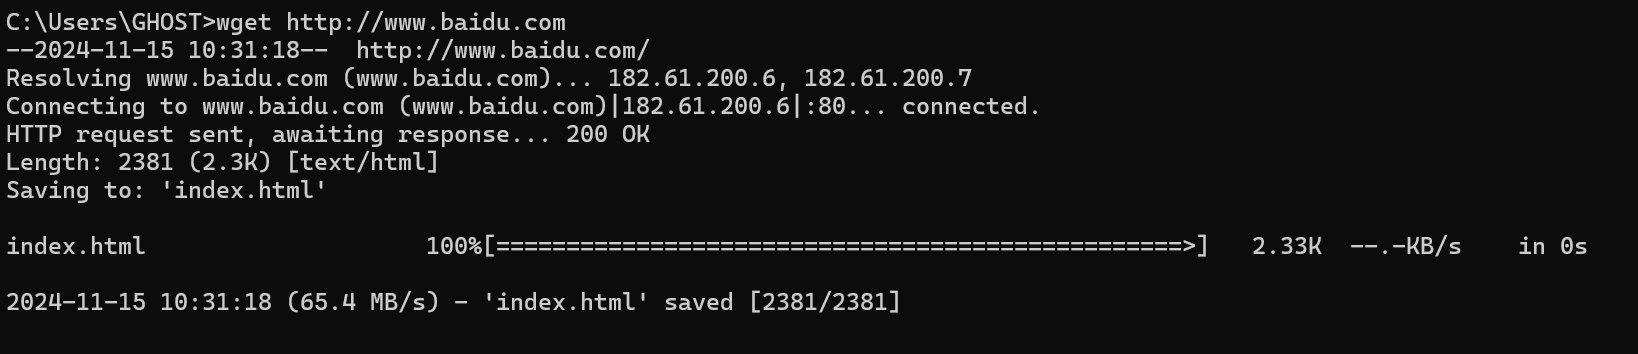
\includegraphics[width=11cm]{images/3.利用wget抓包.png}
		\caption{利用wget抓包}
	\end{figure}
	
	接下来就开始了捕获的过程,如图所示:
	
	\begin{figure}[H]
		\centering
		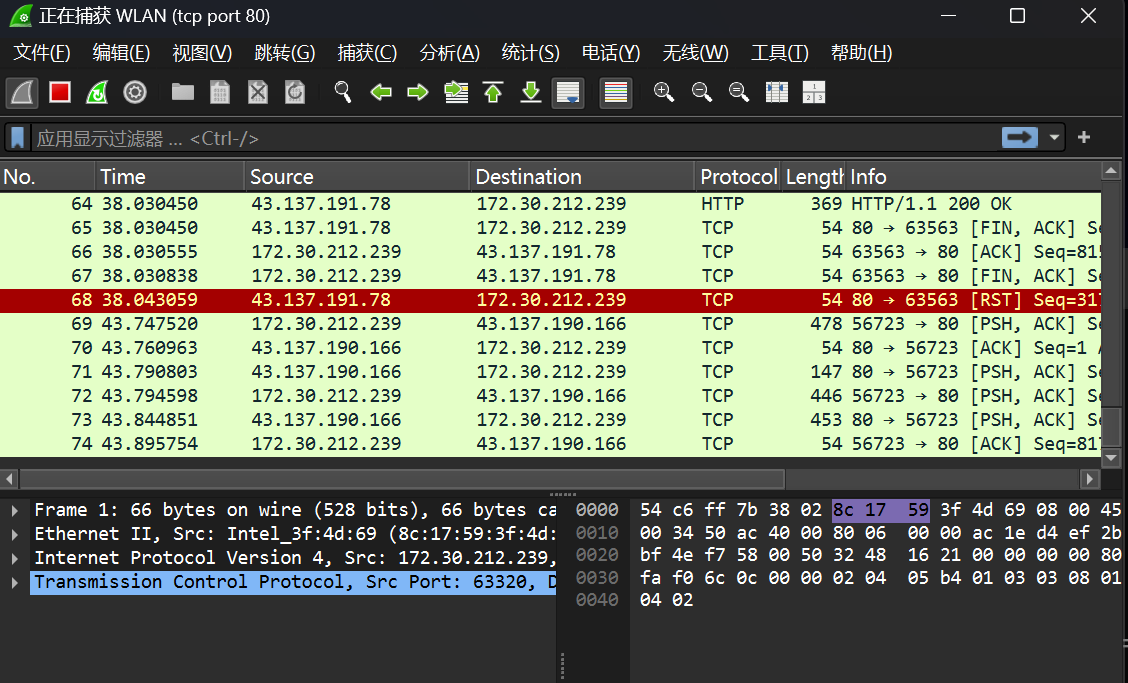
\includegraphics[width=11cm]{images/4.捕获中.png}
		\caption{捕获中}
	\end{figure}
	
	最后,我们在 \texttt{Wireshark} 中停止捕获,得到如下结果:
	
	\begin{figure}[H]
		\centering
		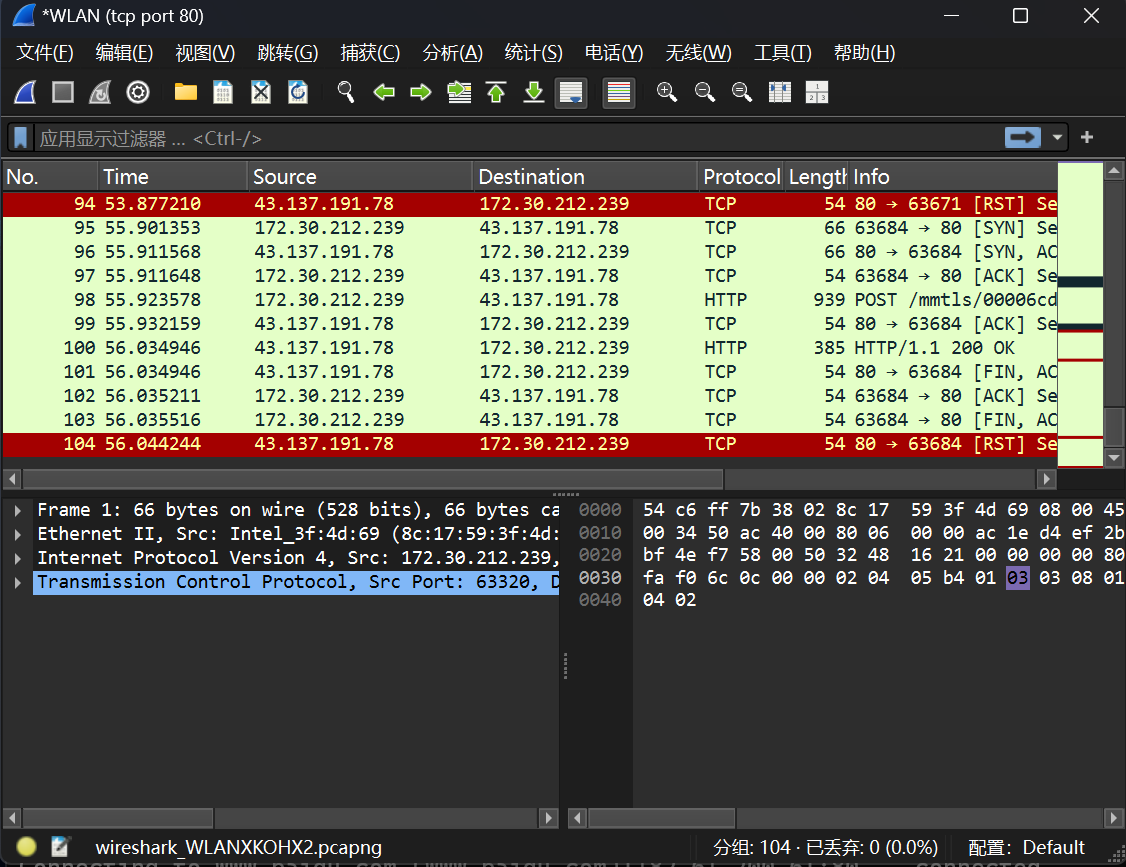
\includegraphics[width=11cm]{images/5.捕获结束.png}
		\caption{捕获结束}
	\end{figure}
	
	\subsection{绘制数据包结构}
	
	接下来,我们分析数据包的结构。在\texttt{Wireshark}中,我们找到了如图的\texttt{HTTP} \texttt{GET}协议包,可以看到其内容,如下图所示:
	
	\begin{figure}[H]
		\centering
		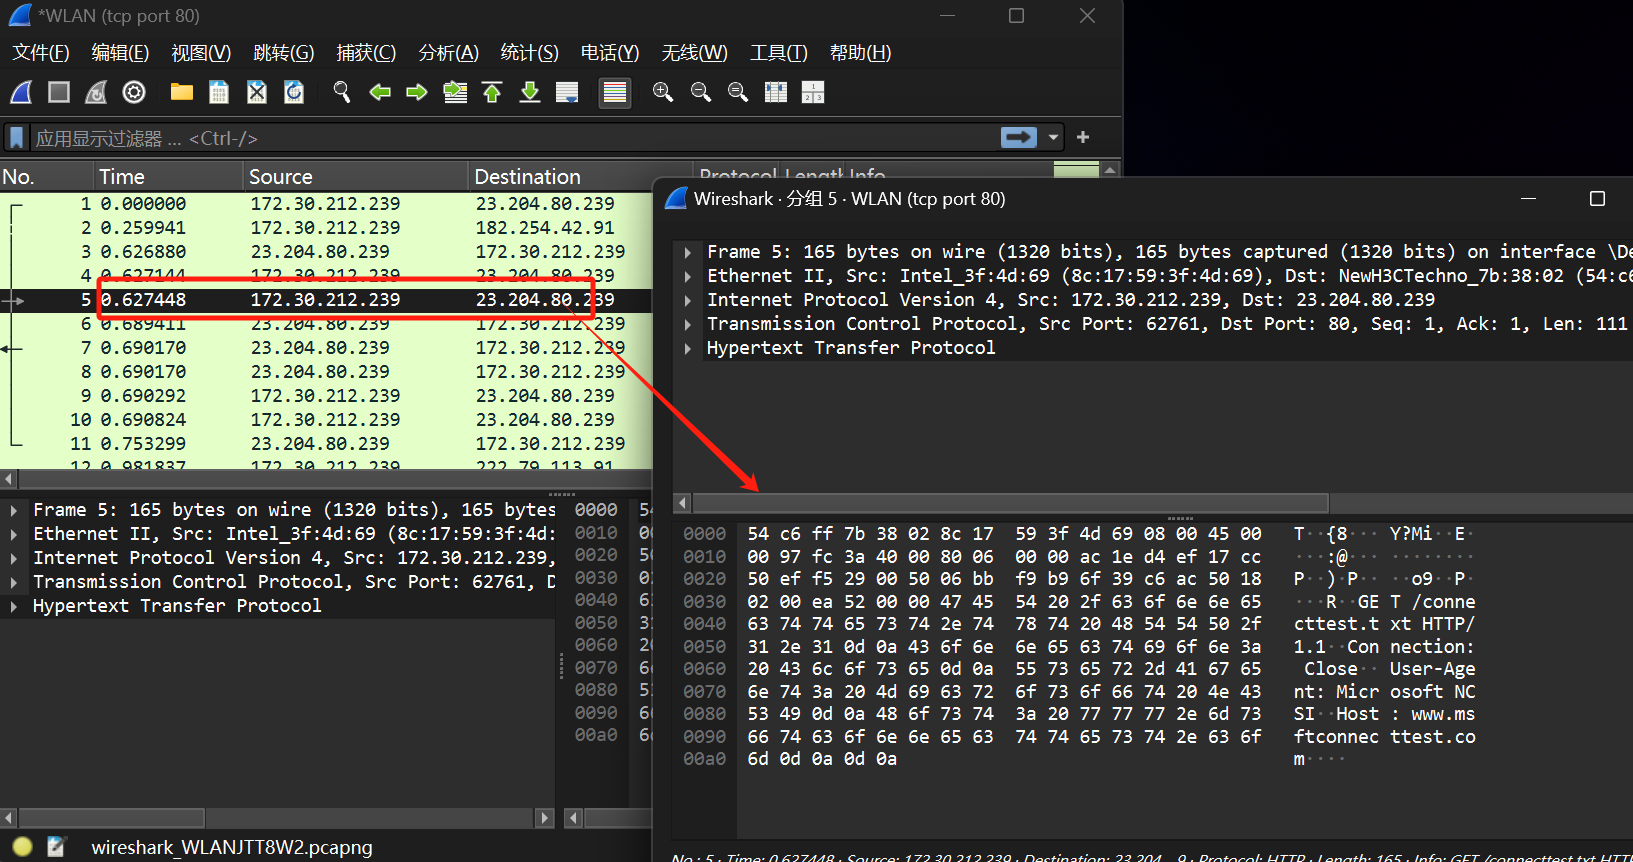
\includegraphics[width=11cm]{images/6.绘制数据包.png}
		\caption{HTTP GET协议包内容}
	\end{figure}
	
	先来大致的查阅一下数据包的结构:
	
	\begin{figure}[H]
		\centering
		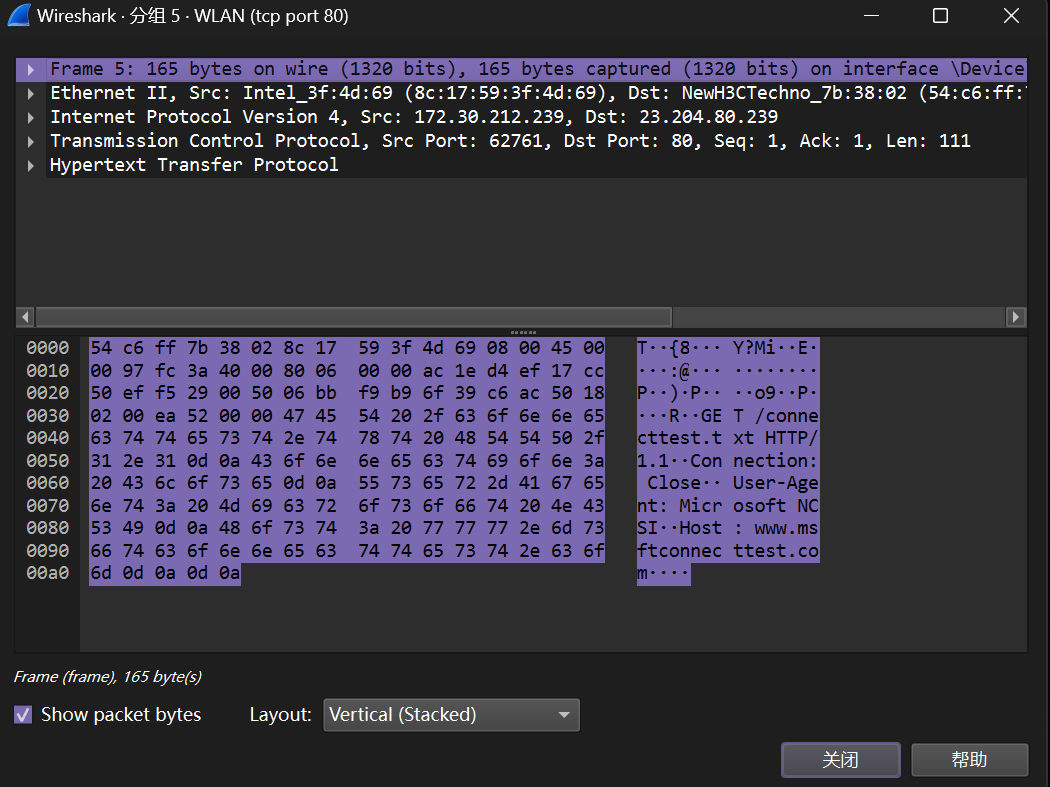
\includegraphics[width=11cm]{images/7.数据包整体信息.png}
		\caption{数据包整体信息}
	\end{figure}
	
	我们可以看到:
	
	第一个块:\texttt{Frame},这不是一个协议,而是一个记录,描述有关数据包的整体信息,包括捕获时间和长度等。我们可以看到,整个数据包的长度是\texttt{165}字节。
	
	第二个块:\texttt{Ethernet II},这是以太网协议,可以看到这个标头的长度是\texttt{14}字节。
	
	第三个块:\texttt{Internet Protocol Version 4},这是\texttt{IP}协议,可以看到这个标头的长度是\texttt{20}字节。
	
	第四个块:\texttt{Transmission Control Protocol},这是\texttt{TCP}协议,可以看到这个标头的长度是\texttt{20}字节。
	
	第五个块:\texttt{Hypertext Transfer Protocol},这是\texttt{HTTP}协议,可以看到这个标头的长度是\texttt{111}字节。
	
	接下来就是每一块的具体内容:
	
	\begin{figure}[H]
		\centering
		\begin{minipage}[b]{0.45\textwidth}
			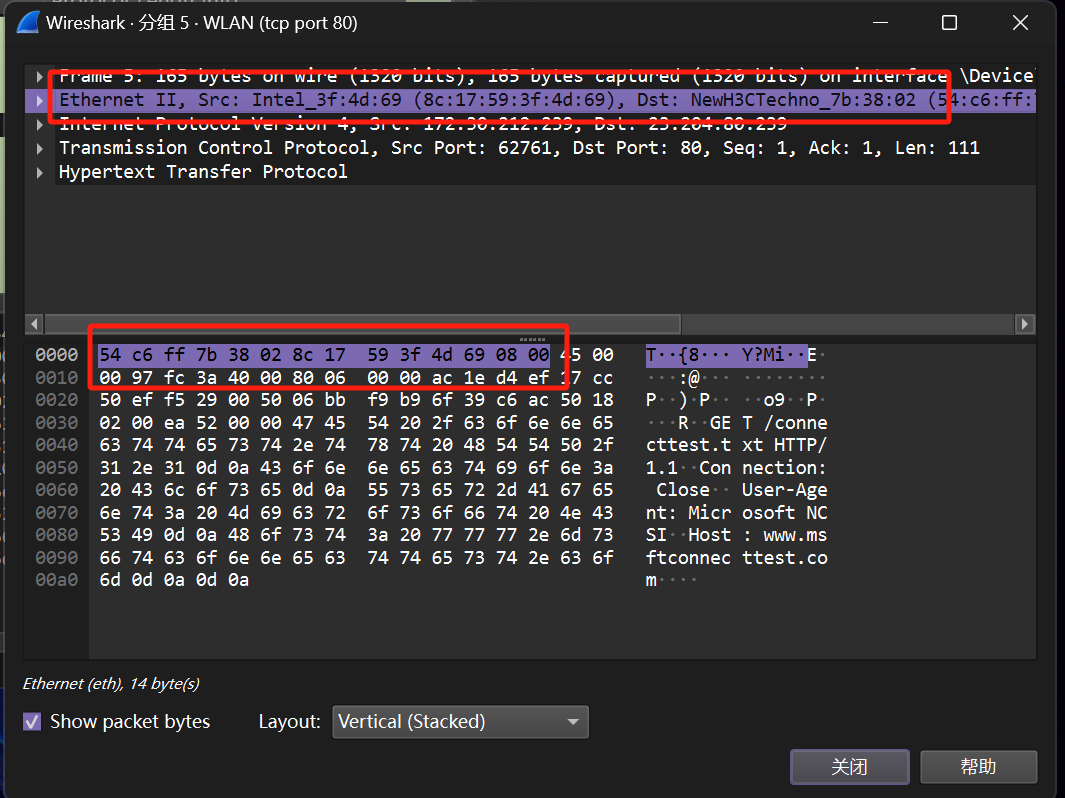
\includegraphics[width=\textwidth]{images/8.以太网数据.png}
			\caption{以太网数据}
		\end{minipage}
		\hfill
		\begin{minipage}[b]{0.45\textwidth}
			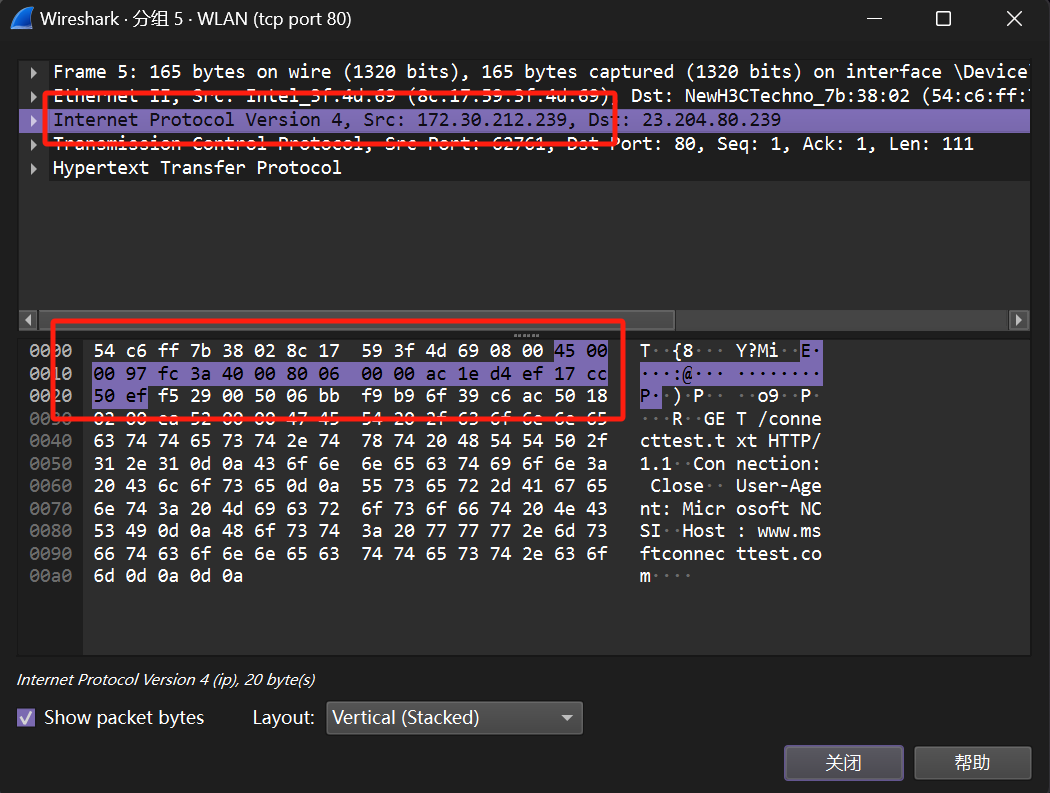
\includegraphics[width=\textwidth]{images/9.IP数据.png}
			\caption{\texttt{IP数据}}
		\end{minipage}
	\end{figure}
	
	\begin{figure}[H]
		\centering
		\begin{minipage}[b]{0.45\textwidth}
			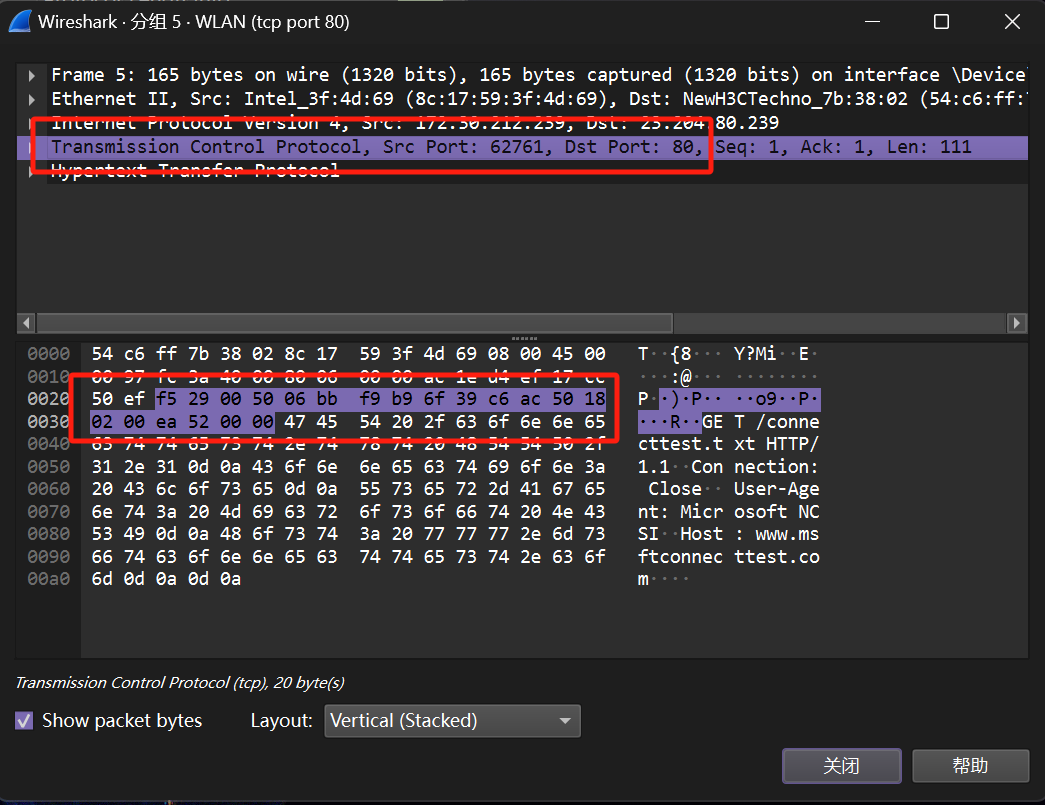
\includegraphics[width=\textwidth]{images/10.TCP数据.png}
			\caption{TCP数据}
		\end{minipage}
		\hfill
		\begin{minipage}[b]{0.45\textwidth}
			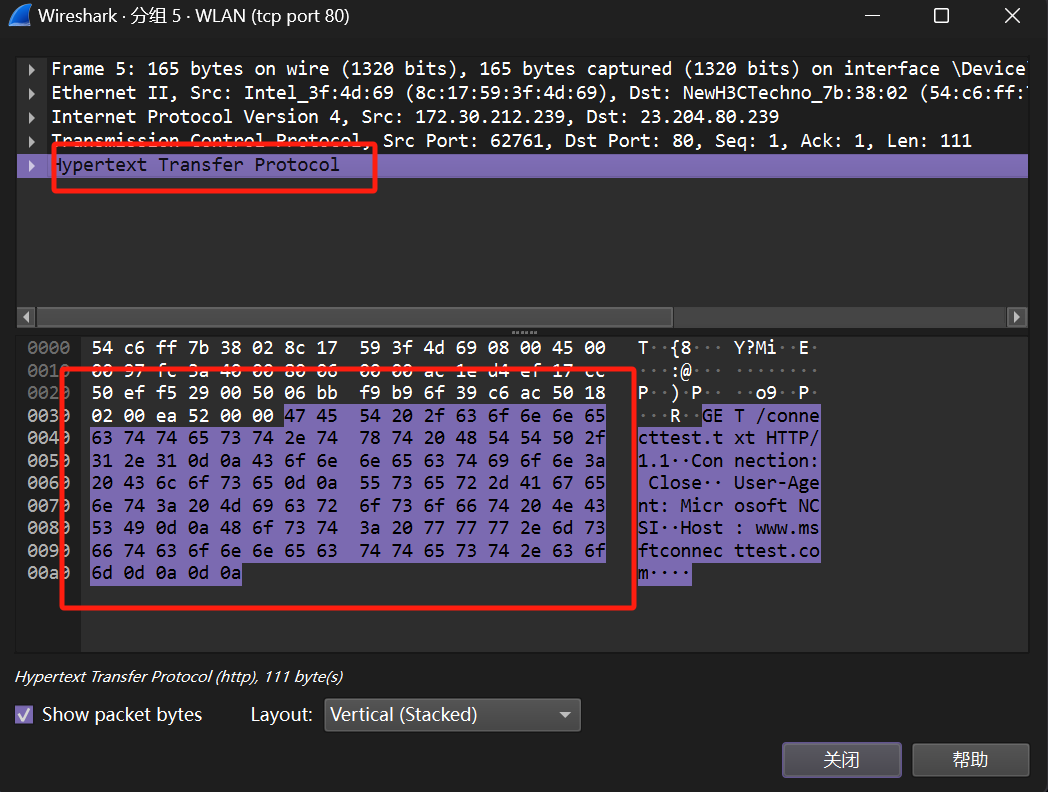
\includegraphics[width=\textwidth]{images/11.HTTP数据.png}
			\caption{\texttt{HTTP数据}}
		\end{minipage}
	\end{figure}
	
	所以由此,绘制的协议包的结构如下图所示:
	
	\begin{figure}[H]
		\centering
		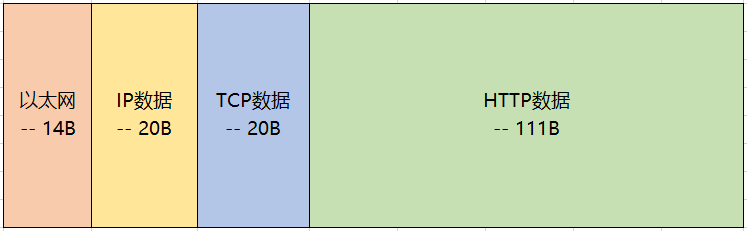
\includegraphics[width=11cm]{images/12.绘制数据协议包.jpg}
		\caption{绘制数据协议包}
	\end{figure}
	
	\subsection{分析协议开销}
	
	\texttt{以太网} 的开销为
	
	$$
	\frac{14}{165}=8.48\%
	$$
	
	\texttt{IP} 的开销为
	
	$$
	\frac{20}{165}=12.12\%
	$$
	
	\texttt{TCP} 的开销为
	
	$$
	\frac{20}{165}=12.12\%
	$$
	
	整个捕获过程(从\texttt{SYN ACK}开始,
	到\texttt{HTTP}后的第一个\texttt{TCP}数据包结束)的开销为
	
	$$
	\frac{14+20+20+66+54+60}{165 + 66 + 54 +60}= 67.82\%
	$$
	
	有用的\texttt{HTTP}数据的开销为
	
	$$
	\frac{111}{165 + 66 + 54 + 60}= 32.17\%
	$$
	
	\begin{figure}[H]
		\centering
		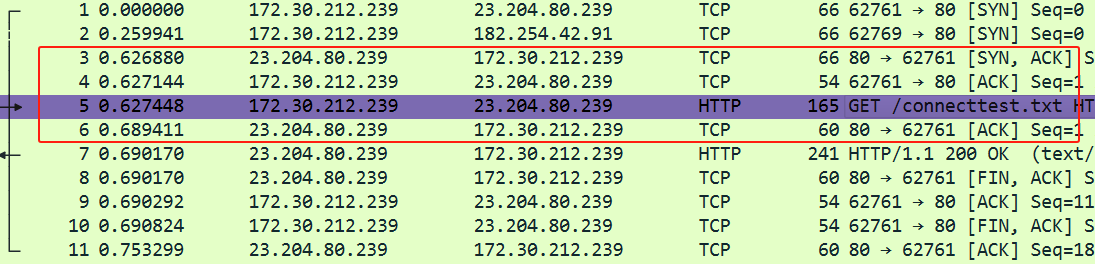
\includegraphics[width=11cm]{images/13.捕获过程.png}
		\caption{整个捕获过程}
	\end{figure}
	
	\subsection{分析解复用键}
	
	\begin{enumerate}[noitemsep]
		\item Which Ethernet header field is the demultiplexing key that tells it the next higher layer is IP? What value is used in this field to indicate \textbf{“IP”}?
		
		\texttt{以太网}头部中的\texttt{type}字段是解复用键,它的值为\texttt{0x0800},表示\texttt{IP}协议。
		
		\item Which IP header field is the demultiplexing key that tells it the next higher layer is TCP? What value is used in this field to indicate \textbf{“TCP”}?
		
		\texttt{IP}头部中的\texttt{protocol}字段是解复用键,它的值为\texttt{0x06},表示\texttt{TCP}协议。
		
	\end{enumerate}
	
	\begin{figure}[H]
		\centering
		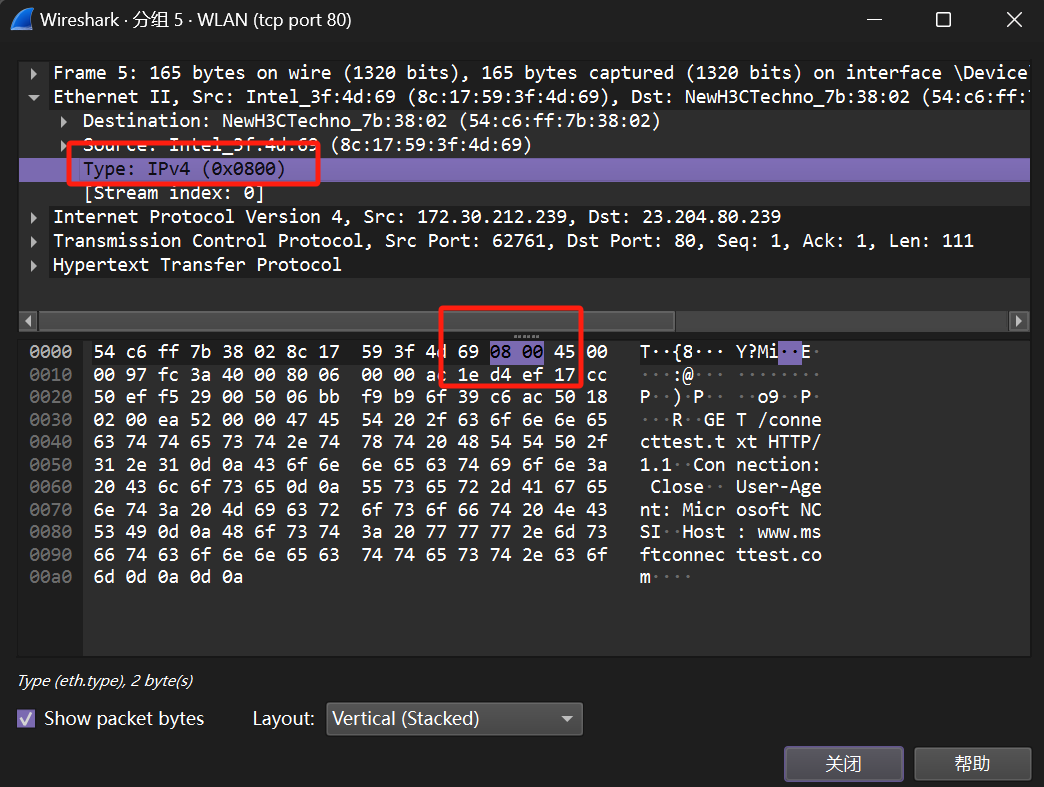
\includegraphics[width=11cm]{images/14.Type字段.png}
		\caption{\texttt{以太网}头部}
	\end{figure}
	
	\begin{figure}[H]
		\centering
		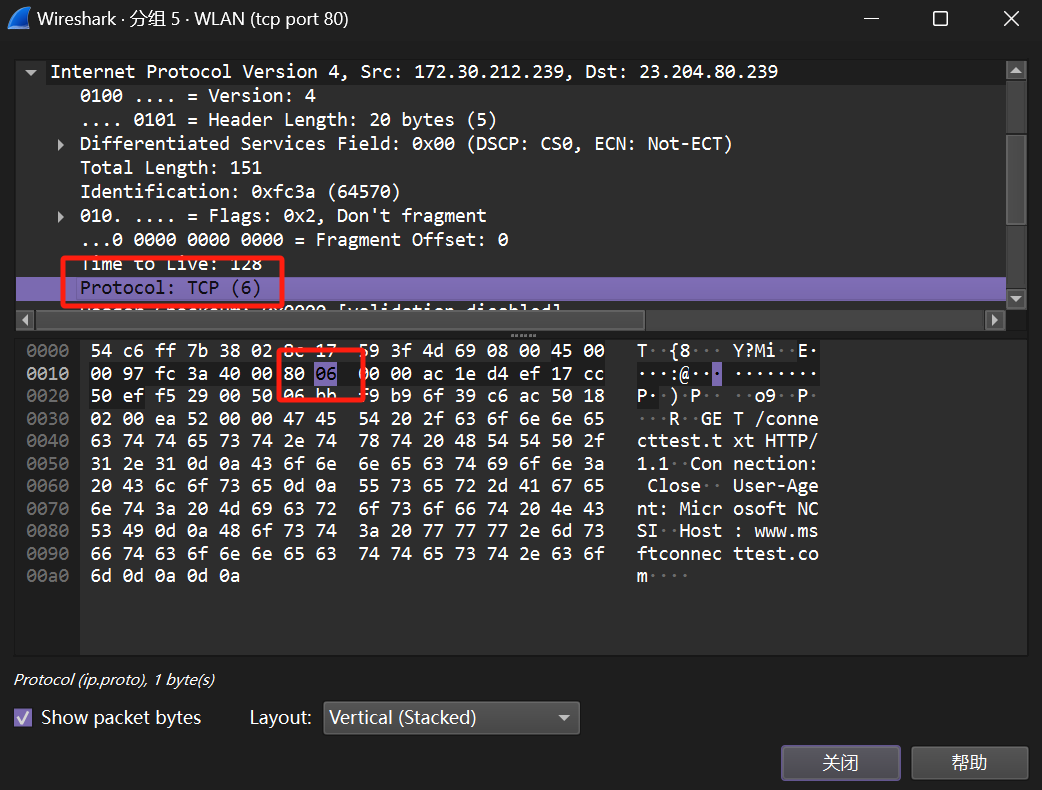
\includegraphics[width=11cm]{images/15.Protocol字段.png}
		\caption{\texttt{IP}头部}
	\end{figure}
	
	\subsection{问题讨论}
	
	\begin{enumerate}[noitemsep]
		\item Look at a short TCP packet that carries no higher-layer data. To what entity is this packet destined? After all, if it carries no higher-layer data then it does not seem very useful to a higher layer protocol such as HTTP!
		
		该数据包的目的地是我们试图访问的网站或我们自己的设备。它主要包含确认和控制信息,对于建立\texttt{TCP}连接至关重要。这类报文是\texttt{TCP}三次握手过程的一部分,对于\texttt{HTTP}协议的运作是必不可少的。
		
		
		\item In a classic layered model, one message from a higher layer has a header appended by the lower layer and becomes one new message. But this is not always the case. Above, we saw a trace in which the web response (one HTTP message comprised of an HTTP header and an HTTP payload) was converted into multiple lower layer messages (being multiple TCP packets).  Imagine that you have drawn the packet structure (as in step 2) for the first and last TCP packet carrying the web response.  How will the drawings differ?
		
		首个\texttt{TCP}数据包携带的是\texttt{HTTP}协议的头部信息,而随后的\texttt{TCP}数据包则承载\texttt{HTTP}协议的有效载荷内容。
		
		\item In the classic layered model described above, lower layers append headers to the messages passed down from higher layers. How will this model change if a lower layer adds encryption?
		
		双方必须就加密算法达成一致,这样在数据传输过程中,接收方才能够正确解密数据。否则,接收方将无法解析数据包中的内容。
		
		\item In the classic layered model described above, lower layers append headers to the messages passed down from higher layers. How will this model change if a lower layer adds compression?
		
		发送方可以在数据包的头部附加解压缩方法的说明,这样接收方在接收到数据包后,便能够先进行解压缩,随后顺利解析数据包中的内容。
		
	\end{enumerate}
	
	\section{实验结果总结}
	
	在本次实验中,我不仅学会了如何使用Wireshark工具捕获不同协议层的数据包,还深入掌握了这些数据包的结构。通过对协议开销的细致分析,我进一步理解了复用键的概念。这些经历极大地加深了我对计算机网络中协议层的理解和认识。
	
	
	\section{附录}
	
	无
	
\end{document}